\chapter{Approche métallurgique }
\label{ch:thermodynamique}

\vfill

Ce chapitre vise à présenter les caractéristiques et les comportements métallurgiques des alliages 16NiCrMo13 et 23MnCrMo5 sous différentes conditions de traitement et d'enrichissement. La Section~\ref{sec:thermocalc} permet de présenter rapidement l'approche CALPHAD et le logiciel Thermo-Calc~\cite{Andersson2002,Borgenstam2000}. Ce logiciel sera ensuite employé dans l'étude des systèmes binaires et ternaires \ch{Fe-C}, \ch{Fe-N} et \ch{Fe-C-N} à la Section~\ref{sec:simple_systems}, qui présente aussi leur description fournie dans la littérature. Quelques résultats concernant le calcul de diagrammes de phase pour des aciers faiblement alliés sont regroupés dans la Section~\ref{sec:low_alloy} avant de procéder dans la Section~\ref{sec:studied_alloys} aux simulations des diagrammes utiles à la compréhension des nuances étudiées. Les compositions nominales en pourcentage massique de ces alliages sont présentées Tableau~\ref{tab:composition_alliages}. Comme il s'agit d'aciers faiblement alliés, la définition des conditions aux limites pour ces simulations demande la connaissance de la thermodynamique des systèmes contenant non seulement fer, carbone et azote mais aussi nickel, chrome, manganèse et molybdène. Des résultats expérimentaux de la littérature sont nécessaires pour une simulation cohérente des systèmes métallurgiques. Ces données de base seront utilisées au cours des discussions conduites au Chapitre~\ref{ch:reponse_metallurgique}. Alors que l'enrichissement des alliages a été effectué dans des conditions favorisant l'équilibre thermodynamique, les caractéristiques mécaniques des traitements de cémentation et carbonitruration résultent d'une trempe et par conséquent d'une transformation hors équilibre du type martensitique. La Section~\ref{sec:martensite_cn} traite des propriétés obtenues et des caractéristiques métallurgiques des structures martensitiques des aciers au carbone et à l'azote. Finalement la Section~\ref{sec:carbonitrurationalliages} présente des résultats relatifs à la réponse métallurgique et mécanique des aciers faiblement alliés aux traitements thermochimiques de cémentation et de carbonitruration. Cela comprend non seulement des aspects relatifs à la structure, mais aussi des aspects liés à la composition locale des couches enrichies.

\begin{table}[!hb]
  \caption{\label{tab:composition_alliages}Composition nominale en pourcentage massique des alliages étudiés.}
  
  \centering{}\footnotesize{}%
  \begin{tabular}{\$c^c^c^c^c^c^c^c}
    \toprule[2pt] 
    \rowstyle{\bfseries}
    Alliage & Fe & C & Si & Mn & Cr & Ni & Mo\tabularnewline
    \midrule[2pt] 
    16NiCrMo13 & bal. & 0,16 & 0,25 & 0,45 & 1,00 & 3,20 & 0,25
    \tabularnewline[6pt] 
    23MnCrMo5 & bal. & 0,23 & 0,25 & 1,30 & 1,20 & 0,10 & 0,25
    \tabularnewline
    \bottomrule
  \end{tabular}
\end{table}

\vfill\clearpage

\section{L'approche CALPHAD et Thermo-Calc}
\label{sec:thermocalc}

Les premiers travaux sur les transformations de phase des aciers faiblement alliés remontent aux années 1930. À partir de ces résultats pionniers, d'énormes progrès ont été réalisés. Ce n'est qu'avec les initiatives de Kaufmann et Ansara, qui sont à l'origine de l'approche CALPHAD~\footnote{Originalement de l'Anglais \textit{CALculation of PHAse Diagrams}, Calcul des Diagrammes de Phase. Aujourd'hui la communauté CALPHAD s'intitule \textit{Computer Coupling of Phase Diagrams and Thermochemistry}, Couplage Numérique du Calcul des Diagrammes de Phase et Thermochimie.}, dans les années 1970 que le calcul des diagrammes de phase avec l'aide d'ordinateurs est devenu populaire~\cite{Spencer2007}. Dans cette méthode, l'énergie de Gibbs de chaque phase est exprimée en fonction de la température, de la composition et, parfois de la pression. À partir de ces données, qui sont généralement issues des mesures expérimentales, l'équilibre est calculé en minimisant numériquement l'énergie libre. Le plus souvent la représentation de ces données thermodynamiques est faite en utilisant des polynômes de Redlich-Kister~\cite{Redlich1948,Hillert2008}. Plusieurs modèles de solution solide sont disponibles pour que l'équilibre soit calculé, parmi lesquels on trouve le modèle classique de Bragg-Williams des solutions strictement régulières~\cite{Hillert2008}. Pour des phases st{\oe}chiométriques le modèle des solutions régulières de \citet{Hillert1970} est le plus connu. Ce sont ces modèles qui sont incorporés dans l'approche CALPHAD que l'on trouve dans le logiciel Thermo-Calc~\cite{Andersson2002,Borgenstam2000} utilisé dans la présente étude. Ce logiciel est utilisé dans la simulation des systèmes thermodynamiques formés par plusieurs groupes de matériaux, sa description détaillée étant disponible dans des publications de \citet{Sundman1985} et \citet{Andersson2002}. L'ouvrage de \citet{Hillert2008} résume globalement les fondements théoriques nécessaires à son utilisation.

Alors que l'utilisation d'un logiciel de ce type permet d'obtenir rapidement des résultats sur les matériaux ou les traitements étudiés, il est aussi facile d'obtenir des informations sans sens physique sur les phénomènes modélisés. Une connaissance préalable des phases possiblement attendues à l'équilibre dans des conditions réalistes de simulation est indispensable avant de procéder à des calculs. Pour cette raison, la suite de ce chapitre est consacrée à réunir des résultats de la littérature permettant une utilisation correcte de Thermo-Calc~\cite{Andersson2002,Borgenstam2000}. L'intérêt principal d'utiliser un logiciel prédisant les équilibres thermodynamiques pour l'étude et la mise au point de traitements thermochimiques est de prédire la formation des précipités qui apparaissent lors du traitement, ce qui induit une consommation des éléments d'alliage de la matrice austénitique que l'on peut observer par microscopie électronique en transmission. Cela permet également de simuler les limites de solubilité des phases dans les alliages en fonction des teneurs en éléments interstitiels et d'estimer les fractions de phases à une température donnée. Il est aussi possible  de déterminer les facteurs thermodynamiques pour le transport à l'état solide. La connaissance des fractions des éléments d'alliage consommés lors de l'enrichissement des matériaux en carbone et principalement en azote est nécessaire pour comprendre d'abord la réponse mécanique \textendash{} en dureté \textendash{} lors de la trempe, et pour estimer ensuite les possibles équilibres de phases lors du revenu. Comme la formation de ces précipités \og piège \fg{} des éléments interstitiels et conduit aussi à appauvrir la matrice en éléments d'alliage, la réponse au revenu des aciers faiblement alliés peut se rapprocher de celle du fer pur, comme cela sera discuté dans la Section~\ref{sec:carbonitrurationalliages}. Ce type de précipitation à haute température produit une barrière à la diffusion du carbone et de l'azote, ce qui peut être traité par Thermo-Calc~\cite{Andersson2002,Borgenstam2000}. En ce qui concerne le contrôle des procédés, le logiciel permet de généraliser les méthodes présentées dans la Section~\ref{sec:procedes} \textendash{} le calcul des diagrammes de température de point de rosée et de potentiel de nitruration \textendash{} pour des systèmes métallurgiques contenant plusieurs composants chimiques. Pour ces simulations, on se servira des bases de données TCFE7, SSOL4, SSUB3 de Thermo-Calc~\cite{Andersson2002,Borgenstam2000}. On peut résumer les applications de cette approche dans ce rapport au calcul:
\begin{itemize}
  \item des diagrammes de phase binaires,
  \item des sections pseudo-binaires des alliages,
  \item des sections isothermes des alliages,
  \item des diagrammes de potentiel de nitruration,
  \item des diagrammes de température de point de rosée, et
  \item des profils de diffusion-précipitation.
\end{itemize}

\section{Équilibre des phases: résultats de la littérature}
\label{sec:low_alloy_literature}

\subsection{Systèmes modèles: \ch{Fe-C}, \ch{Fe-N} et \ch{Fe-C-N}}
\label{sec:simple_systems}

La description des alliages à base de fer commence avec celles des systèmes connus les plus simples : les diagrammes d'équilibre \ch{Fe-C}, \ch{Fe-N} et \ch{Fe-C-N}. En fait, pour des raisons cinétiques, l'équilibre \ch{Fe-C} n'est normalement pas atteint et le système représentatif pour les aciers est en fait celui du diagramme binaire métastable \ch{Fe-Fe3C}~\cite{Mittemeijer2010} dans lequel le carbone se trouve soit en solution solide avec le fer \textendash{} de limite de solubilité très faible à basse température \textendash{} soit sous forme de cémentite. Ce diagramme (Figure~\ref{fig:binaire_fe_c}) présente les domaines monophasés de la ferrite de structure cubique centrée (CC) connue comme phase $\alpha$ et stable à basse température, de l'austénite $\gamma$ cubique face centrée (CFC) stable à des températures intermédiaires, de la cémentite \ch{Fe_{3}C} et de la phase $\delta$ qui est aussi \og{}CC\fg{} comme la phase $\alpha$ mais se situe près de la température de fusion et dont l'importance technologique est limitée. La simulation de ce diagramme a été réalisée avec les bases de données TCFE7 et SSOL4 conduisant à des résultats assez similaires en termes de domaines de phase représentés graphiquement sur la Figure~\ref{fig:binaire_fe_c}.

Pour la cémentation, les frontières entre les domaines $\alpha+\gamma$ ($\mathrm{A_{3}}$) et $\gamma+\ch{Fe3C}$ ($\mathrm{A_{cm}}$) avec le domaine monophasé de l'austénite sont d'une importance cruciale : la première frontière détermine la température minimale pour conduire le traitement \textendash{} une ligne équivalente peut être calculée pour les systèmes faiblement alliés \textendash{} tandis que la seconde fixe la fraction massique en carbone pour atteindre la saturation de l'austénite et est donc liée au contrôle des atmosphères d'enrichissement. C'est l'activité du carbone sur cette limite $\mathrm{A_{cm}}$ qu'on a calculée à la Section~\ref{sec:controle_cementation}, pour laquelle on observe Figure~\ref{fig:binaire_fe_c} une limite de solubilité dans l'austénite de l'ordre de $w_{s,C}\approxeq0,013$ dans la plage de température typique de la carbonitruration. Cette saturation de l'austénite conduit à la formation de carbures du type \ch{Fe3C}. Si l'on considère encore ce diagramme pour prédire le comportement lors d'un revenu réalisé à \SI{573}{\kelvin} après une trempe, c'est encore \ch{Fe3C} qui est le carbure d'équilibre.

\begin{figure}[h]
  \centering
  \subfloat[\label{fig:binaire_fe_c}\ch{Fe-Fe3C}]{
    \centering
    \resizebox{0.48\textwidth}{!}{
      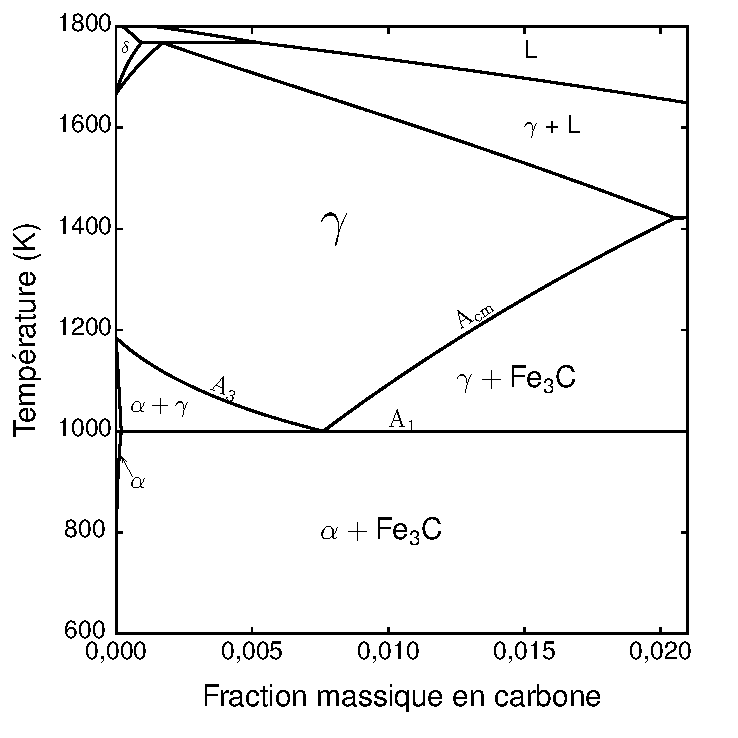
\includegraphics{figures/ch-02-diagram_fe_cem}}
  }\hfill
  \subfloat[\label{fig:binaire_fe_n}\ch{Fe-N}]{
    \centering
    \resizebox{0.48\textwidth}{!}{
      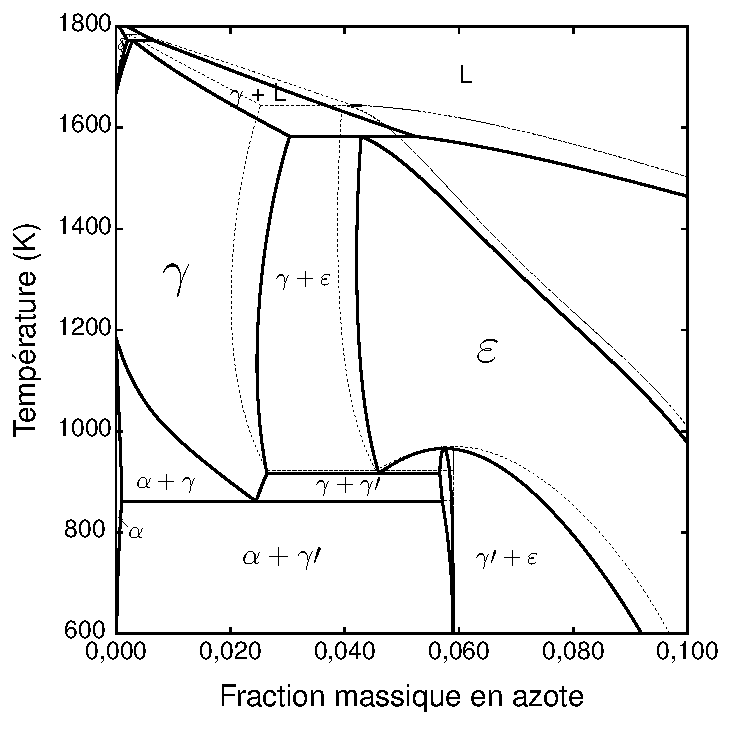
\includegraphics{figures/ch-02-diagram_fe_n}}
  }
  
  \caption{\label{fig:binaires_fe}Diagrammes binaires des systèmes \protect\subref{fig:binaire_fe_c} \ch{Fe-Fe3C} et \protect\subref{fig:binaire_fe_n} \ch{Fe-N}. Thermo-Calc~\cite{Andersson2002,Borgenstam2000}. Traits pleins base de données SSOL4, pontillés TCFE7. Les résultats pour les deux bases de données se superposent dans le diagramme \ch{Fe-Fe3C}.}
\end{figure}

Dans le cas du système \ch{Fe-N} les phases $\alpha$, $\gamma$ et $\delta$ constituent les domaines monophasés \textendash{} avec l'azote comme élément en solution interstitiel \textendash{} auxquels il faut ajouter $\gamma\prime$, phase intermétallique \ch{Fe4N_{(1-x)}} non-st{\oe}chiométrique de structure \og{}CFC\fg{} et $\varepsilon$, intermétallique \ch{Fe2N_{(1-x)}} non-st{\oe}chiométrique de structure hexagonale compacte \og{}HC\fg{}~\cite{Frisk199179,Du1993,Gantois2010}. La Figure~\ref{fig:binaire_fe_n} présente les phases en équilibre de \SIrange{600}{1800}{\kelvin}. On observe dans ce cas des résultats distincts selon la base de données utilisée, notamment une réduction du domaine monophasé $\gamma$ pour la base de données TCFE7, pour laquelle le nitrure \ch{Fe4N} est aussi considéré comme étant st{\oe}chiométrique. Dans la plage de températures employées pour la carbonitruration, l'allure de ce diagramme est semblable à celle observée dans le système \ch{Fe-Fe3C}. Comme pour le système \ch{Fe-Fe3C}, deux lignes dans le diagramme sont particulièrement importantes pour les traitements en phase austénitique : la limite $\alpha+\gamma/\gamma$ détermine la température minimale pour le procédé tandis que la frontière $\gamma/\gamma+\varepsilon$ donne la saturation en azote, qui est située au-delà de la saturation en carbone dans ce cas (une fraction massique de l'ordre de 0,025 en azote).

Pour le système ternaire \ch{Fe-C-N}, les mêmes configurations que celles trouvées dans les binaires sont possibles, auxquelles il faut ajouter la présence des domaines biphasés $\ch{Fe3C}+\varepsilon$ et $\alpha+\varepsilon$, comme cela est exposé dans \citet{Gantois2010}. En faisant un parallèle avec la discussion conduite sur l'étape de revenu dans le système \ch{Fe-Fe3C}, on s'attend à une précipitation de \ch{Fe4N_{(1-x)}} à \SI{573}{\kelvin} pour le système \ch{Fe-N}. Bien que cette phase soit observée expérimentalement, la formation de nitrures intermédiaires de type \ch{Fe16N2}~\cite{Liu2000} est amplement rapportée dans la littérature~\cite{Kaplow1983,vanGent1985,Mittemeijer1988,Cheng199013,Cheng19902857,Fall1996,vanGenderen1997,Sherby2008}. Ces nitrures se forment lors du vieillissement à température ambiante et se décomposent en \ch{Fe4N_{(1-x)}} lors du revenu des alliages \ch{Fe-N}. On reviendra sur ce sujet au Chapitre~\ref{ch:reponse_metallurgique}.

À partir de cette compilation de résultats, et pour simuler les systèmes \ch{Fe-C} et \ch{Fe-N} dans les conditions qui nous intéressent pour les traitements thermochimiques, il faut retenir les phases~\footnote{En raison des modèles de solution utilisés dans le formalisme CALPHAD, les phases à considérer dans une simulation sont décrites par leurs structures cristallines et par les différents sites disponibles dans les réseaux. Cela implique normalement que l'on doit fournir à Thermo-Calc~\cite{Andersson2002,Borgenstam2000} les structures selon leurs nomenclatures utilisées par ces bases de données et non nécessairement par leurs nomenclatures d'usage.} suivantes dans les calculs d'équilibre:
\begin{itemize}
  \item $\alpha$, allotropie \og{}CC\fg{} du fer stable à la température ambiante,
  \item $\gamma$, structure \og{}CFC\fg{} présente à partir de \SI{1000}{\kelvin},
  \item \ch{Fe3C}, la cémentite, carbure de fer, et
  \item les nitrures de types \ch{Fe4N_{(1-x)}} et \ch{Fe2N_{(1-x)}}.
\end{itemize}

\subsection{Alliages réels: aciers faiblement alliés}
\label{sec:low_alloy}

La connaissance des systèmes présentés Section~\ref{sec:simple_systems} est indispensable à la compréhension des traitements de cémentation et de carbonitruration, les phases requises pour les simuler faisant aussi partie de l'ensemble nécessaire pour les simulations d'équilibres dans les aciers. Il s'avère toutefois que l'introduction d'éléments d'alliage dans les aciers faiblement alliés déplace les domaines des diagrammes de phases et introduit de nouvelles phases possibles à l'équilibre. On s'intéresse donc aux alliages de fer contenant des atomes de \ch{Cr}, \ch{Ni}, \ch{Mo}, \ch{Mn}, \ch{Si}, \ch{C} et \ch{N}, du type de ceux décrits au Tableau~\ref{tab:composition_alliages}. Dans un premier temps, on s'intéresse aux résultats de la littérature qui peuvent nous permettre de simuler l'état d'équilibre dans des alliages réels.
 
La simulation de l'état d'équilibre dans des alliages requiert la connaissance préalable des phases qui possiblement peuvent constituer le système. Cette limitation de l'approche CALPHAD est intrinsèquement liée aux modèles de solution et à leur représentation polynomiale: c'est en minimisant l'énergie libre des solutions décrites par des modèles structuraux pré-définis que les phases à l'équilibre sont établies. De cette manière, l'approche reste semi-empirique. D'autres méthodes disponibles pour le calcul des diagrammes de phase, telles que les méthodes \textit{ab initio} et les méthodes d'approximation quantique sont aussi disponibles~\cite{Bozzolo2007} mais leur emploi demande une étude spécifique des systèmes en question que nous n'avons pas réalisée. On trouve aussi un intérêt à utiliser ces approches plus fondamentales pour obtenir des données nécessaires à l'approche CALPHAD, ce qui réduit le besoin de données expérimentales~\cite{Bozzolo2007}.
 
Dans ce cadre semi-empirique, on cherchera dans cette section à déterminer quels sont les carbures et nitrures stables dans la plage de températures pour l'enrichissement en carbone et en azote des alliages étudiés. Ensuite, on s'intéressera non seulement à la séquence de précipitation, mais aussi à la distribution des éléments d'alliage dans les carbures et nitrures formés à basse température en condition de revenu. L'introduction d'éléments d'alliage ayant une affinité supérieure à celle du fer pour le carbone et l'azote implique la formation de différents types de carbures et de nitrures, en lieu et place de ceux formés à partir du fer uniquement~\cite{Steel2006}. À partir des coupes isothermes pour les systèmes  \ch{Fe-Mo-C}~\cite{Chatfield1977} et  \ch{Fe-Mn-C}~\cite{Hillert197797} on vérifiera que pour les teneurs en éléments d'alliage du Tableau~\ref{tab:composition_alliages}, le carbure associé à la saturation en carbone lors de l'étape de cémentation est certainement du type \ch{Fe3C} pour les deux alliages. Cela a été confirmé récemment par \citet{Djurovic2011479}. Lors du revenu, la précipitation de carbures de type \ch{M23C6}~\cite{Kuo1985991} est probable~\footnote{Lorsque les carbures formés sont alliés, on utilise la lettre \ch{M} pour représenter les atomes occupant les sites associés aux éléments métalliques faisant partie de ces réseaux.}. En considérant l'analyse des systèmes ternaires \ch{Fe-Cr-C}~\cite{Benz1974} et quaternaires \ch{Fe-Cr-Ni-C}~\cite{Hillert19912187}, on observe que pour les compositions considérées, le carbure stable devrait aussi être du type \ch{M3C}. Dans le cas où les alliages sont plus riches en \ch{Cr} et \ch{Mo}, la description du système \ch{Fe-Cr-Mo-C} faite par \citet{Hillert1992} s'avère utile. \citet{Raghavan1992} montre pour le système \ch{Fe-Cr-C-N} le besoin de considérer aussi l'équilibre de l'austénite avec des carbures \ch{M23C6} et \ch{M7C3} à la température d'enrichissement dans des alliages avec plus de 0,7\% de chrome en poids. 

Le nickel, en tant qu'élément non-carburigène, ouvre le domaine de phase austénitique à des températures moins élevées~\cite{Steel2006}. Le système \ch{Fe-Cr-Mn-C}~\cite{Lee1993} suggère aussi que des carbures du type \ch{M7C3}  devraient faire partie des phases à considérer pour les simulations d'équilibre des alliages étudiés. Dans le coin riche en fer des systèmes contenant \ch{Cr}, \ch{Mo} et \ch{Mn}, ces atomes de substitution ont pour effet principal de stabiliser le carbure \ch{M23C6} et déplacent la composition eutectoïde vers des valeurs plus faibles en carbone. Le chrome favorise quant à lui la formation de nitrures du type \ch{MN}, pour lesquels le chrome est toujours l'élément prépondérant~\cite{Steel2006}. La limite de solubilité en carbone doit être réduite en raison de la présence d'éléments carburigènes. Ces éléments jouent aussi un rôle dans leur répartition entre la matrice et les précipités. Dans le cas de l'azote, cette réduction doit être beaucoup plus prononcée, comme dans le cas de l'équilibre pour le système \ch{Fe-Cr-N}~\cite{Raghavan1987}. Le Tableau~\ref{tab:phases_retenir} résume les phases à retenir dans la simulation des alliages étudiés avec leur composition possible selon la base de données TCFE7 de Thermo-Calc~\cite{Andersson2002,Borgenstam2000}. Bien que \citet{Catteau2016} rapportent la présence de nitrures du type \ch{MnSiN2}~\cite{Weitzer1987178} dans l'alliage 23MnCrMo5 enrichi en azote, il n'a pas été possible de l'insérer dans les simulations en raison de l'absence de données thermodynamiques. \citet{Weitzer1987178} fournissent une description de ce système mais les paramètres thermodynamiques ne sont pas fournis pour utilisation avec l'approche CALPHAD.

\begin{table}
  \caption{\label{tab:phases_retenir}Phases à retenir pour la simulation d'équilibre des phases des alliages 16NiCrMo13 et 23MnCrMo5. Le carbure \ch{M3C} peut être substitué à l'azote et le nitrure \ch{MN} est décrit par le même réseau de l'austénite dans la base de données TCFE7.}
  
  \centering{}\footnotesize{}%
  \begin{tabular}{\$l^l}
    \toprule[2pt] 
    \rowstyle{\bfseries}
    Phase & Description\tabularnewline
    \midrule[2pt] 
    $\alpha$    & Ferrite, solution de \ch{Cr,\,Fe,\,Mn,\,Mo,\,Ni,\,Si}
    \tabularnewline[6pt]
    $\gamma$    & Austénite, solution de \ch{Cr,\,Fe,\,Mn,\,Mo,\,Ni,\,Si}
    \tabularnewline[6pt]
    \ch{M3C}    & Cémentite alliée, M = (\ch{Cr,\,Fe,\,Mn,\,Mo,\,Si})
    \tabularnewline[6pt]
    \ch{M23C6}  & Carbure substitué, M = (\ch{Cr,\,Fe,\,Mn,\,Mo,\,Ni})
    \tabularnewline[6pt]
    \ch{M7C3}   & Carbure substitué, M = (\ch{Cr,\,Fe,\,Mn,\,Mo,\,Ni,\,Si})
    \tabularnewline[6pt]
    \ch{MN}     & Nitrure \ch{CrN} substitué, M = (\ch{Cr,\,Fe,\,Mn,\,Mo,\,Ni,\,Si})
    \tabularnewline[6pt]
    \ch{MnSiN2} & Nitrure mixte de manganèse-silicium\tabularnewline
    \bottomrule
  \end{tabular}
\end{table}

\section{Simulation des alliages étudiés}
\label{sec:studied_alloys}

Avant de procéder à l'analyse des profils de diffusion et des réponses mécaniques induites, il est utile de connaître l'équilibre local des phases à la fin d'un cycle de traitement \textendash{} juste avant la trempe \textendash{} le long des profils en carbone et en azote. Pour cela, le logiciel Thermo-Calc~\cite{Andersson2002,Borgenstam2000} a été utilisé pour simuler les coupes pseudo-binaires et isothermes à la température de traitement des alliages étudiés \textemdash{} Tableau~\ref{tab:composition_alliages}. Ces simulations considèrent comme états de référence pour le carbone et l'azote, le graphite et \ch{N2} à la pression atmosphérique, respectivement. Les phases compilées dans le Tableau~\ref{tab:phases_retenir} sont considérées dans ces simulations. On doit remarquer, lorsque les simulations prennent en compte plus de trois éléments d'alliage, que les conodes des diagrammes ne se trouvent plus dans le plan des coupes pseudo-binaires et isothermes et seuls les seuils de précipitation des carbures et des nitrures peuvent être déterminés graphiquement~\cite{Hillert2008}. Des informations additionnelles, comme la répartition des phases en domaines multi-phasés, demandent des  calculs spécifiques pour la composition requise.

\subsection{Diagrammes pseudo-binaires}

En tenant compte des résultats de la littérature et des simulations des systèmes simplifiés présentées précédemment, on peut établir des coupes pseudo-binaires en fonction de la fraction massique en carbone des alliages 16NiCrMo13 et 23MnCrMo5 à l'aide de Thermo-Calc~\cite{Andersson2002,Borgenstam2000}, Figure~\ref{fig:pseudo_binaires}. Cela permet d'identifier la limite de solubilité en carbone lorsque les autres éléments sont fixés pour la condition de traitement, dans la plage de températures typiquement employée pour les traitements thermochimiques, mais aussi de prédire les différents précipités attendus lors du revenu. Les deux nuances présentent de grandes similitudes entre elles en ce qui concerne le domaine austénitique $\gamma$. La température de l'eutectoïde est environ \SI{50}{\kelvin} inférieure pour la nuance 16NiCrMo13 (Figure~\ref{fig:aero_pseudo_binaire}) du fait de la présence de nickel. Cependant, cette température augmente légèrement pour la nuance 23MnCrMo5 (Figure~\ref{fig:auto_pseudo_binaire}) si on la compare à celle du système \ch{Fe-C} (Figure~\ref{fig:binaire_fe_c}). Par rapport à ce diagramme modèle \ch{Fe-C}, les coupes ont la même allure à haute température avec l'apparition des domaines multi-phasés pour les équilibres des carbures que l'on ne retrouve pas dans le fer pur de types \ch{M23C6} et \ch{M7C3}. Le carbure \ch{M23C6} est le principal carbure prédit pour l'alliage 16NiCrMo13 en dessous d'une fraction massique en carbone de 0,006 qui est la valeur recherchée en surface \textendash{} teneur à partir de laquelle la formation d'austénite résiduelle $\gamma_{R}$ est favorisée \textendash{} dans les traitements de cémentation et de carbonitruration. Ce n'est pas le cas pour l'alliage 23MnCrMo5, lequel favorise la précipitation de \ch{M7C3}. En comparant les bases de données SSOL4 et TCFE7, on observe une grande similitude entre les simulations pour les faibles teneurs en carbone et pour le domaine $\gamma$. Alors que les mêmes carbures sont prédits par les deux bases, les domaines peuvent être décalés en fraction en carbone ou en température et des domaines supplémentaires peuvent être présents.

\begin{figure}[h]
  \centering
  \subfloat[\label{fig:aero_pseudo_binaire}16NiCrMo13]{
    \centering\resizebox{0.48\textwidth}{!}{
      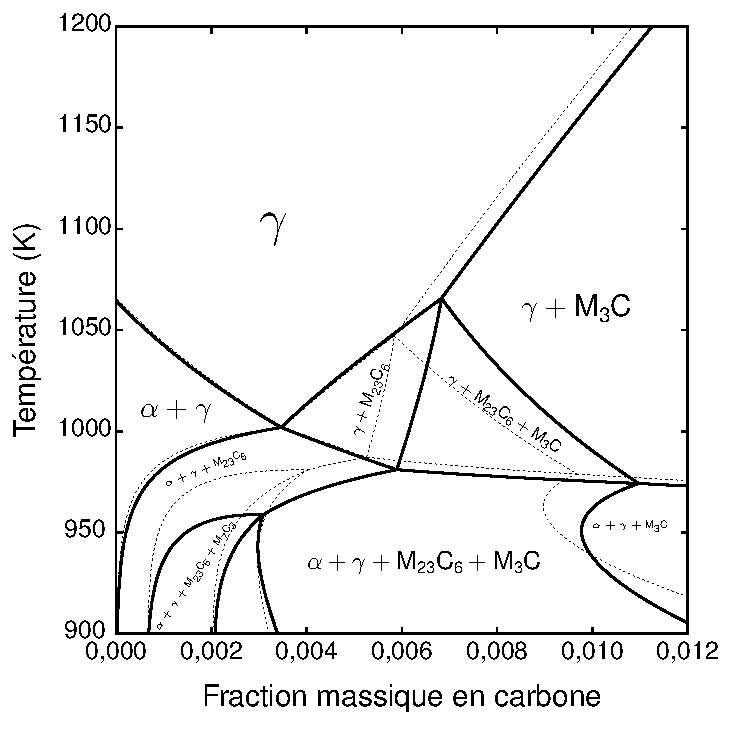
\includegraphics{figures/ch-02-diagram_pseudo_bin_aero}}
  }\hfill
  \subfloat[\label{fig:auto_pseudo_binaire}23MnCrMo5]{
    \centering\resizebox{0.48\textwidth}{!}{
      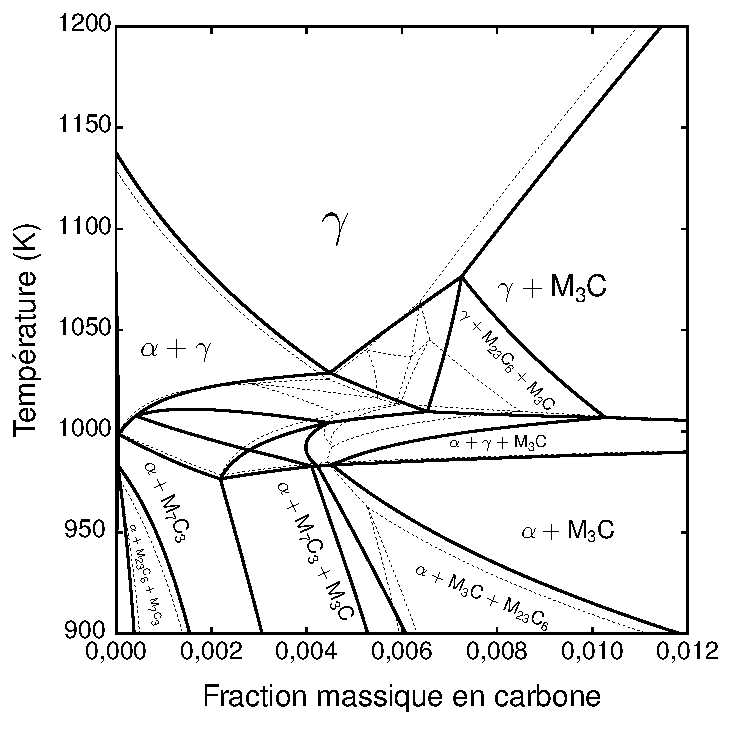
\includegraphics{figures/ch-02-diagram_pseudo_bin_auto}}
  }
  
  \caption{\label{fig:pseudo_binaires}Diagrammes pseudo-binaires établis en fonction de la fraction massique en carbone des alliages \protect\subref{fig:aero_pseudo_binaire} 16NiCrMo13 et \protect\subref{fig:auto_pseudo_binaire} 23MnCrMo5. Résultats obtenus avec Thermo-Calc~\cite{Andersson2002,Borgenstam2000}. Traits pleins base de données SSOL4, pontillés TCFE7.}
\end{figure}

Pour les deux nuances, la fraction massique en carbone permettant d'atteindre la saturation en surface dans la plage allant de \SIrange{1143}{1213}{\kelvin} se situe entre 0,009 et 0,011 et varie linéairement.  Les deux diagrammes de la Figure~\ref{fig:pseudo_binaires} montrent une réduction de la fraction massique en carbone pour la transformation de décomposition de l'austénite \textendash{} le point équivalent à la transformation eutéctoïde dans le système \ch{Fe-C} \textendash{} ce qui résulte de l'augmentation de l'activité de cet élément en présence des éléments d'alliage: la précipitation des carbures est favorisée. Dans tous les cas, en ce qui concerne l'enrichissement en carbone, les diagrammes montrent une limite de solubilité en carbone assez proche et les réponses en enrichissement aux conditions de cémentation et de carbonitruration au-delà de \SI{1150}{\kelvin} doivent rester similaires. Lors du revenu, les précipitations de cémentite alliée \ch{M3C} et de carbures \ch{M23C6} sont attendues pour des fractions massiques en carbone allant de 0,003 à 0,006, teneurs typiquement recherchées dans les couches traitées.

Des coupes pseudo-binaires établies en fonction de la fraction massique en azote sont tracées Figure~\ref{fig:pseudo_binaires_azote}. Ces diagrammes ne présentent plus de grandes similitudes avec leurs équivalents dans le système \ch{Fe-N}. Cela est dû a la présente d'éléments nitrurigènes, notamment le chrome, qui conduisent à la formation de nitrures \ch{MN} dans la plage de composition considérée. Pour des faibles teneurs en azote ($w_{N}\le 0,002$) le carbure prépondérant à basse température dans chaque alliage \textendash{} \ch{M23C6} pour la nuance 16NiCrMo13 et \ch{M7C3} pour 23MnCrMo5 \textendash{} se trouve à l'équilibre avec le nitrure \ch{MN}. En augmentant la teneur en azote, on observe simultanément la diminution de la température de transformation austénitique et le remplacement de ces carbures par la cémentite alliée. La phase \ch{Si3N4} est possible selon la base de données TCFE7. Cette phase ne sera pas considérée en raison de sa lente cinétique de précipitation à faible teneur en \ch{Si} dans les alliages \textendash{} cette phase est typiquement observée dans les aciers au silicium où la fraction en \ch{Si} dépasse 0,015.

\begin{figure}[!ht]
  \centering
  \subfloat[\label{fig:aero_pseudo_binaire_azote}16NiCrMo13]{
    \centering\resizebox{0.48\textwidth}{!}{
      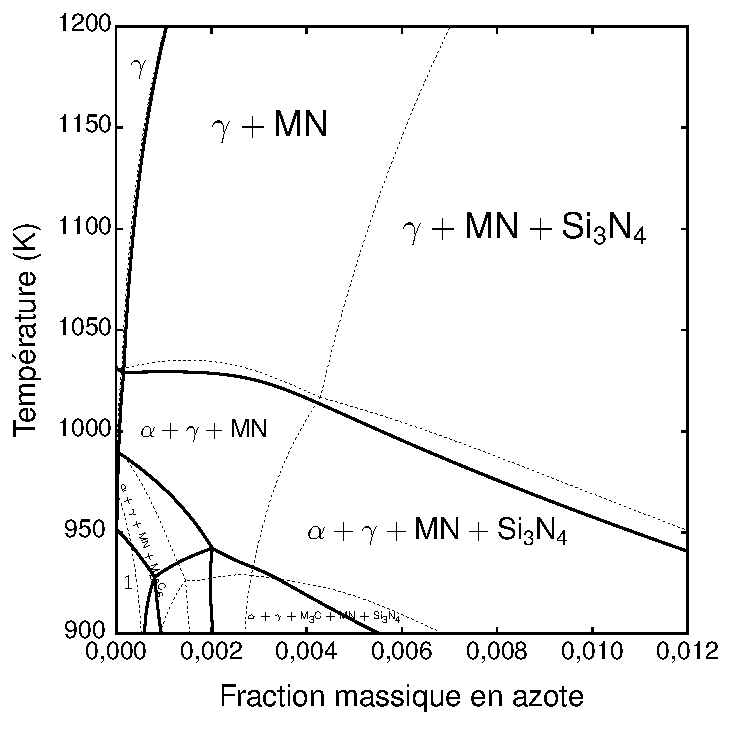
\includegraphics{figures/ch-02-diagram_pseudo_bin_aero_nitro}}
  }\hfill
  \subfloat[\label{fig:auto_pseudo_binaire_azote}23MnCrMo5]{
    \centering\resizebox{0.48\textwidth}{!}{
      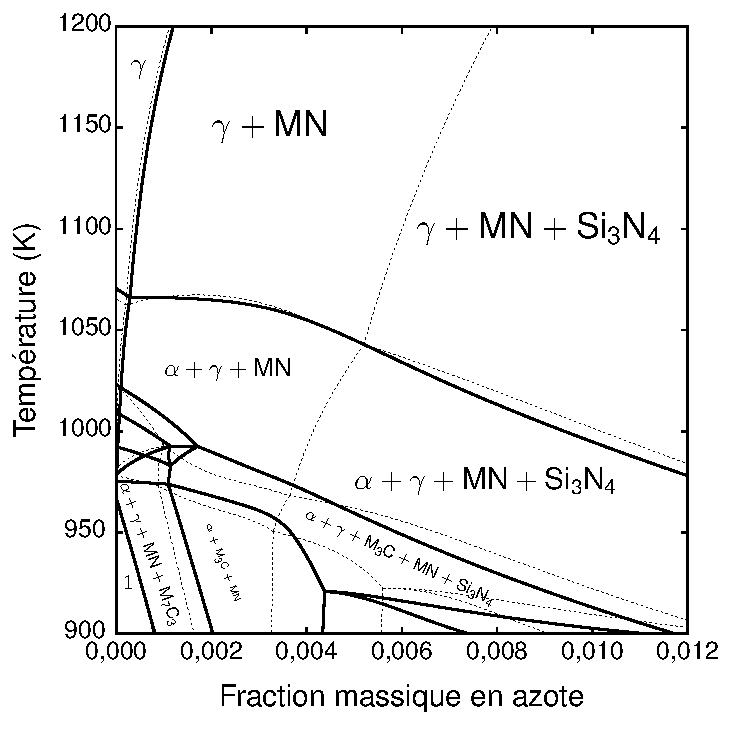
\includegraphics{figures/ch-02-diagram_pseudo_bin_auto_nitro}}
  }

  \caption{\label{fig:pseudo_binaires_azote}Diagrammes pseudo-binaires  établis en fonction de la fraction massique en azote des alliages \protect\subref{fig:aero_pseudo_binaire_azote} 16NiCrMo13 et \protect\subref{fig:auto_pseudo_binaire_azote} 23MnCrMo5. Résultats obtenus avec  Thermo-Calc~\cite{Andersson2002,Borgenstam2000}. Traits pleins base de données SSOL4, pontillés TCFE7.}
\end{figure}

\subsection{Coupes isothermes}

Bien que les diagrammes pseudo-binaires soient utiles à prédire les phases formées lors de la saturation et le comportement d'alliage pendant le refroidissement, des coupes isothermes peuvent être aussi utilisées pour le contrôle des procédés pendant la phase d'enrichissement. La Figure~\ref{fig:isothermes} présente des diagrammes établis en fonction des fractions en carbone et azote simulés à \SI{1173}{\kelvin} pour les deux alliages de cette étude. La limite de solubilité en azote \textendash{} une fraction massique inférieure à 0,001, à partir de laquelle des nitrures substitués de st{\oe}chiométrie \ch{MN} sont précipités \textendash{} s'avère être très peu dépendante de la fraction massique en carbone, lequel sature l'austénite autour de 0,01. La saturation en carbone conduit, pour les deux nuances, à la formation de cémentite alliée dans la région \og{}1\fg{}, des diagrammes, comme cela se voit également dans la Figure~\ref{fig:pseudo_binaires}. Les régions \og{}2\fg{} et \og{}3\fg{} ne présentent aucun intérêt dans le cas présent.

\begin{figure}[!bh]
  \centering
  \subfloat[\label{fig:isothermal_aero}16NiCrMo13]{
    \centering\resizebox{0.48\textwidth}{!}{
      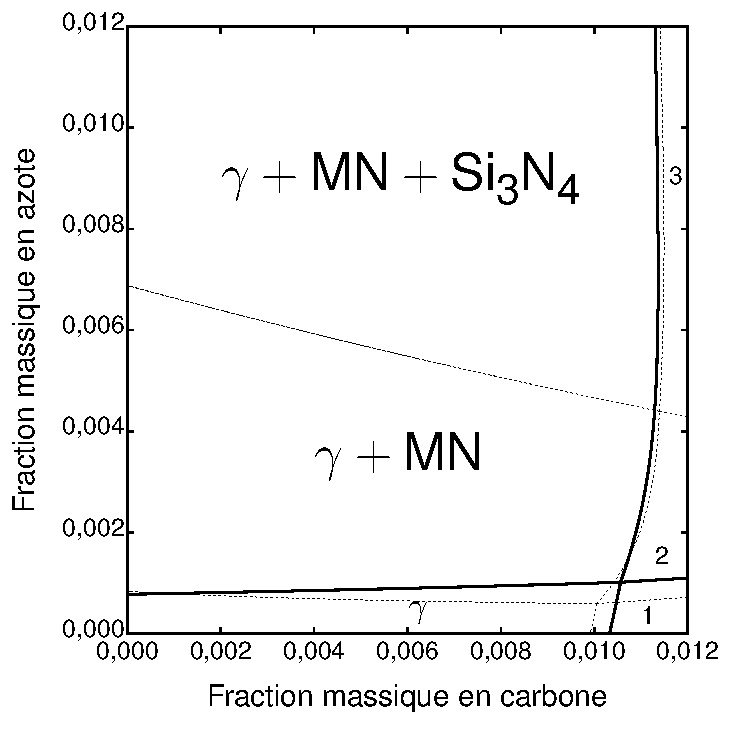
\includegraphics{figures/ch-02-diagram_isothermal_aero}}
  }\hfill
  \subfloat[\label{fig:isothermal_auto}23MnCrMo5]{
    \centering\resizebox{0.48\textwidth}{!}{
      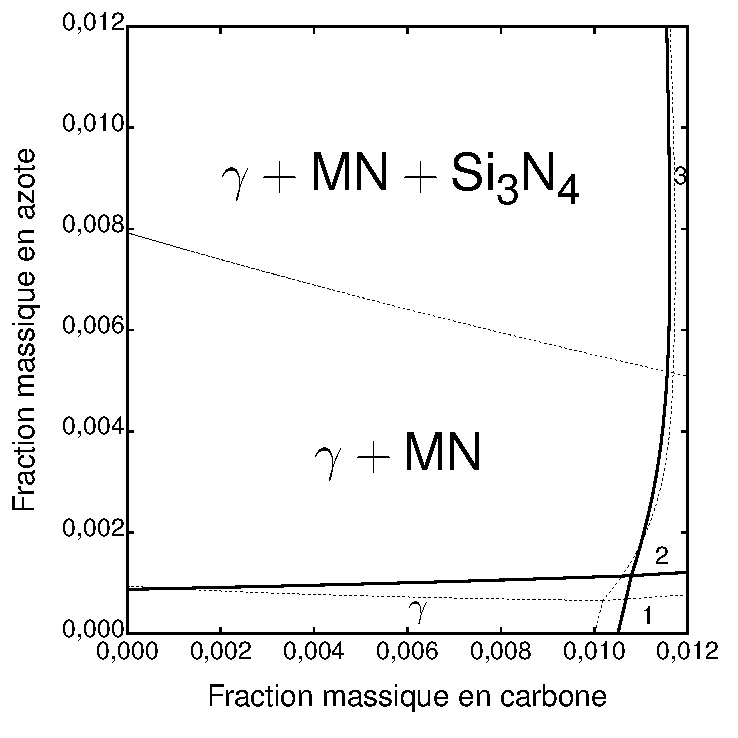
\includegraphics{figures/ch-02-diagram_isothermal_auto}}
  }

  \caption{\label{fig:isothermes}Coupes isothermes à \SI{1173}{\kelvin} établies en fonction des fractions massiques en carbone et azote des alliages \protect\subref{fig:isothermal_aero} 16NiCrMo13 et \protect\subref{fig:isothermal_auto} 23MnCrMo5. Résultats obtenus avec Thermo-Calc~\cite{Andersson2002,Borgenstam2000}. Traits pleins base de données SSOL4, pontillés TCFE7.}
\end{figure}

Comme lors des phases de cémentation, la condition à la limite pour le carbone correspond à une saturation en carbone de la surface dans l'austénite, la précipitation de cémentite n'est donc pas prise en compte \textemdash{} on suppose que la formation et solution de \ch{M3C} est instantanée et la phase n'est pas utilisée dans la simulation. Cela rend possible de réaliser la simulation sans adopter un modèle d'homogénéisation et donc plus rapidement. En revanche, les fractions massiques en azote visées au-delà de 0,003, introduites dans les alliages par la carbonitruration et la nitruration austénitique, impliquent la précipitation de nitrures du type \ch{MN} et un appauvrissement en éléments d'alliage, notamment le chrome et le molybdène, de la matrice austénitique.  Pour tenir compte de cette précipitation et de ses effets, il faut recourir à la Figure~\ref{fig:consommation_matrice} qui montre la consommation du chrome conduisant à la formation des nitrures \ch{MN}. On observe l'évolution de l'azote en solution solide en fonction de la teneur totale dans l'alliage. Jusqu'à la limite de solubilité, la pente des courbes de la Figure~\ref{fig:consommation_azote} est unitaire. Ensuite, les courbes suivent un chemin qui dépend de la composition de l'alliage. Des résultats similaires sont obtenus avec les bases de données TCFE7 et SSOL4. Comme les matériaux sont traités pendant une durée suffisamment longue pour supposer un équilibre des phases, l'azote ainsi calculé sera considéré comme étant représentatif de la composition de la martensite.% obtenue lors de la trempe.

\begin{figure}[h]
  \centering
  \subfloat[\label{fig:consommation_chrome}Chrome en solution solide.]{
    \centering\resizebox{0.48\textwidth}{!}{
    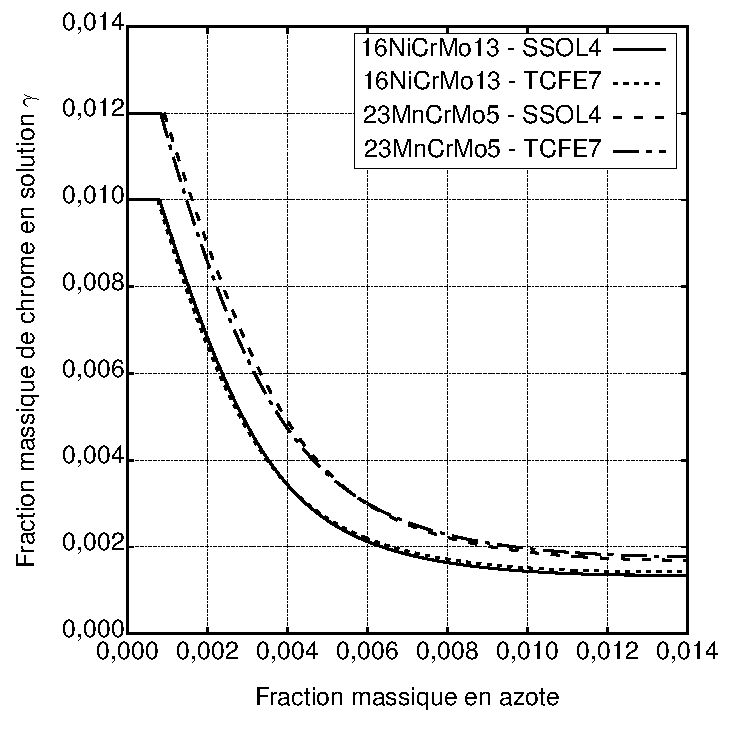
\includegraphics{figures/ch-02-consommation_alliage}}
  }\hfill\subfloat[\label{fig:consommation_azote}Azote en solution solide.]{
    \centering\resizebox{0.48\textwidth}{!}{
    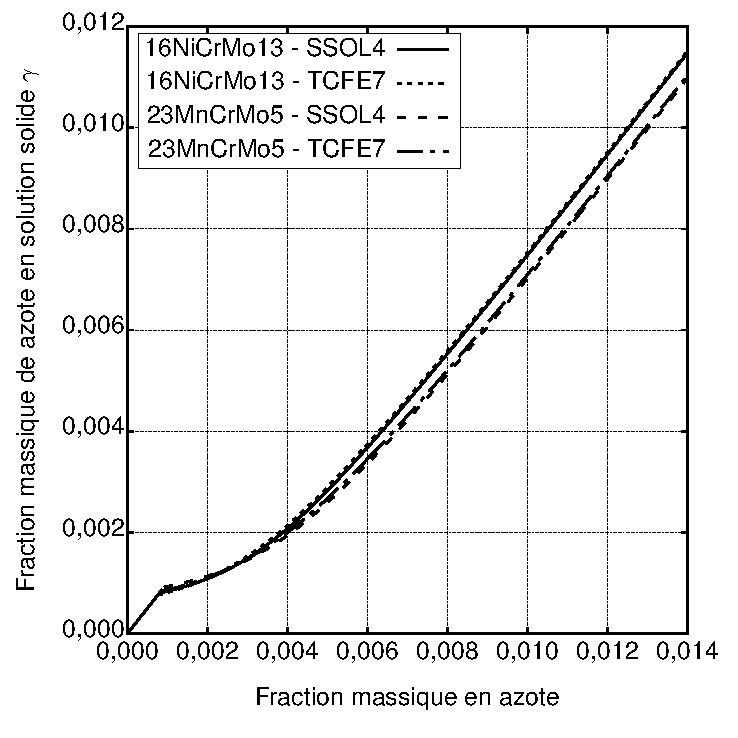
\includegraphics{figures/ch-02-consommation_azote}}
  }

  \caption{\label{fig:consommation_matrice}Simulation de la consommation des éléments en solution solide et formation de nitrures à \SI{1173}{\kelvin}. Résultats obtenus avec Thermo-Calc~\cite{Andersson2002,Borgenstam2000}, bases de données SSOL4 et TCFE7.}
\end{figure}

Les principales caractéristiques des alliages étudiés à retenir, établies au cours de la Section~\ref{sec:studied_alloys} à l'aide de Thermo-Calc~\cite{Andersson2002,Borgenstam2000}, peuvent être résumées ainsi:
\begin{itemize}
  \item les seuils de précipitation de cémentite en domaine $\gamma$ à \SI{1173}{\kelvin} correspondent à des fractions massiques de l'ordre de 0,01. Cependant, l'activité associée à cette valeur \textendash{} en utilisant le graphite comme état de référence \textendash{} n'est pas la même pour les deux nuances. Pour les simulations d'enrichissement, la valeur simulée pour chaque nuance doit être utilisée comme condition à la limite si l'on désire considérer une condition de précipitation de \ch{Fe3C} en surface;
  \item on s'attend à la formation de nitrures du type \ch{MN} pendant l'enrichissement en azote, ce qui doit advenir pour des fractions massiques de cet élément de l'ordre de 0,001. Cette précipitation produit un appauvrissement de la matrice de l'alliage que doit favoriser un comportement au revenu plus proche de celui du système \ch{Fe-C-N}. 
\end{itemize}

\section{Métallurgie de la carbonitruration}
\label{sec:metallurgie_cn}

Les sections précédentes ont principalement abordé le cas de l'équilibre des systèmes métallurgiques étudiés et donc précisent les phases formées pendant l'enrichissement en carbone et en azote. Cette étape est nécessaire pour le contrôle des procédés thermochimiques car elle sert à connaître les seuils de précipitation des nitrures et des carbures, ainsi que l'appauvrissement en éléments d'alliage dans les matrices enrichies. Maintenant, il convient de discuter du comportement des alliages au cours des étapes conférant les propriétés finales à partir des compostions établies par l'enrichissement. La martensite au carbone et à l'azote sera d'abord traitée avant que soient abordées les réponses au revenu des aciers faiblement alliés contenant ces éléments interstitiels.

\subsection{La martensite au carbone et à l'azote}
\label{sec:martensite_cn}

L'obtention des propriétés mécaniques désirées après les traitements thermochimiques dans le domaine austénitique résulte généralement d'une séquence de trempe et revenu. Cela implique une transformation de type martensitique pendant la trempe~\cite{Steel2006}, qui par contraction thermique, dépasse le seuil de contraintes requis pour former la martensite~\cite{Khachaturyan1983}. L'approche mécanique de ce genre de transformation est décrite dans une publication classique de \citet{Kurdjumov1976}. Beaucoup de travaux sont disponibles dans la littérature sur la martensite au carbone des aciers faiblement alliés et sur ses transformations pendant le revenu. Un travail de référence de \citet{Krauss1999} compile de manière concise les propriétés et structures attendues dans des situations rencontrées dans les traitements thermochimiques.

Si l'on considère les enrichissements en carbone dans la plage de 0,005-0,006 en fractions massiques, on doit s'attendre à observer la formation d'une microstructure martensitique en lattes pour des taux de refroidissement typiques~\cite{Krauss1999}. Cette morphologie n'est pas seulement dépendante de la composition \textendash{} ponctuelle dans les traitements thermochimiques \textendash{} et donc de la température $M_{s}$ de début de transformation martensitique, mais aussi de la température à laquelle la transformation s'est passée, laquelle peut être influencée par le milieu de trempe~\cite{Umemoto1983}. Du fait de son caractère fragile, cette martensite est normalement soumise au revenu avant l'utilisation des pièces trempées. Le revenu de la martensite au carbone peut être appréhendé à partir de la plage de température et du traitement thermique appliqué. De manière plus générale, il intègre l'histoire thermique de la pièce après la réalisation de la trempe et donc comprend même les transformations issues des étapes du traitement cryogénique ainsi que le vieillissement à la température ambiante. Dans ce contexte, \citet{Cheng1988} décrivent la suite de transformations qui ont lieu dans la martensite \ch{Fe-C}, suite qui est affectée par la présence d'éléments d'alliage dont l'effet principal est de décaler la plage des températures de chaque régime, notamment en ce qui concerne la transformation des carbures intermédiaires. \citet{Morra2001} fournissent données des cinétiques de ces processus pour quelques aciers.

Dans le cas de la martensite à l'azote, un nombre très limité de publications est disponible~\cite{Catteau2014,Catteau2016}. La littérature est centrée sur le système \ch{Fe-N}, pour lequel les transformations métallurgiques induites par les étapes de revenu et de vieillissement à la température ambiante sont connues~\cite{Kaplow1983,vanGent1985,Mittemeijer1988,Cheng199013,Cheng19902857,Fall1996,vanGenderen1997,Sherby2008}. La formation du nitrure intermédiaire \ch{Fe16N2} a lieu à température ambiante après une centaine d'heures de vieillissement, ce qui apporte une augmentation de la résistance mécanique de la martensite \ch{Fe-N}. Avec le revenu, ce nitrure cohérent devient incohérent et donc la résistance supplémentaire qu'il apporte n'est pas conservée. Bien que comportement, \emph{i.e.} dureté, après trempe de la martensite au carbone puisse être directement décrit par la teneur interstitielle~\cite{Cohen1968,Norstrom1976,Krauss1999,Hutchinson20115845}, le rôle de l'azote n'est pas explicité. 

Pour des faibles teneurs en azote, \citet{Briant1982} montre que cet élément peut induire une fragilisation pendant le revenu. De plus, pour les aciers faiblement alliés, en raison de la formation de nitrures à la température d'enrichissement, la martensite obtenue diffère de la composition de l'alliage de départ, et est plus proche de celle du système \ch{Fe-N}. \citet{Cheng1992} comparent le revenu d'une martensite mixte au carbone et à l'azote (\ch{Fe-C-N}) à celui des systèmes binaires \ch{Fe-C} et \ch{Fe-N}. Les auteurs~\cite{Cheng1992} concluent que la présence simultanée des deux interstitiels accélère la décomposition \ch{Fe16N2 -> Fe4N} et retarde celles des carbures intermédiaires en cémentite et de l'austénite résiduelle, lesquels restent métastables à des températures plus élevées. L'azote en solution solide réduit également la vitesse critique de refroidissement pour la trempe \textendash{} augmentation de la trempabilité de l'alliage. Néanmoins, l'austénite résiduelle est une réalité dans les aciers et sa transformation finale en martensite n'est normalement pas complète~\cite{Steel2006}.

\citet{Norstrom1976} a proposé un modèle pour prédire la limite élastique de la martensite en fonction de sa morphologie et de sa teneur en carbone (Équation~\ref{eq:norstrom_model}). Cette équation prend en compte la friction interne dans le fer pur $\sigma_{0}$, la contribution des éléments d'alliage $\sigma_{1}$, deux termes de Hall-Petch pour incorporer les tailles $d$ des lattes et $D$ des paquets de martensite, la densité intrinsèque de dislocations dans le fer pur martensitique $\rho_{0}$ et son augmentation avec la teneur en carbone $K(C)$.

\begin{equation}
  \sigma_{y}=\sigma_{0}+\sigma_{1}+\frac{k_{y}}{D^{\nicefrac{1}{2}}}
    +\frac{k_{s}}{d^{\nicefrac{1}{2}}}+
    \alpha{Gb}\biggr[\rho_{0}+K(C)\biggr]^{\nicefrac{1}{2}}
  \label{eq:norstrom_model}
\end{equation}

La dépendance du dernier terme de l'Équation~\ref{eq:norstrom_model} avec la racine carrée de la densité de dislocations avait déjà été proposée par \citet{Cohen1968} et trouve ses bases physiques dans la mécanique des dislocations~\cite{Haasen19962009,Hutchinson20115845}. Comme la densité des dislocations augmente de manière linéaire avec la teneur en carbone~\cite{Krauss1999,Morito20031475}, on peut vérifier la validité de cette approche en traçant la résistance mécanique en fonction de la racine carrée de la teneur en interstitiels. Ce modèle reste applicable jusqu'à la transformation de la martensite cubique en martensite quadratique connue sous l'appellation \og{} point-H \fg{}~\cite{Sherby2008}. 
Selon \citet{vanGent1985} la teneur limite en azote pour la transformation de la martensite de cubique à quadratique se situe à une fraction massique d'environ 0,002. Cette valeur n'est pas en accord avec celle rapportée par \citet{Sherby2008} qui la situent à une fraction atomique de 0,0275 pour le carbone et pour l'azote. L'utilisation des fractions atomiques semble plus raisonnable dans ce cas étant donné le caractère du phénomène physique mis en jeu: l'occupation des sites interstitiels produisant une déformation quadratique du réseau cristallin. Cette valeur en fraction atomique correspond à une fraction massique en carbone de 0,006 et en azote de 0,0075.

Bien que $\sigma_{y}$ dépende de plusieurs facteurs comme la morphologie de la martensite, le durcissement par solution solide et la densité et la mobilité des dislocations~\cite{Krauss1999}, la dépendance la plus marquée est celle relative à la teneur en interstitiels en solution solide. Cela permet une comparaison directe entre les matériaux de base fer~\cite{Grange1977,Hutchinson20115845}. \citet{Hutchinson20115845} montrent, par exemple, que pour les nuances~\footnote{Ici rapportées en pourcentages massiques.} Fe-1,7Mn-0,23Si-0,12C et Fe-1,7Mn-0,21Cr-0,23Si-0,23C la contribution des éléments d'alliage dans l'Équation~\ref{eq:norstrom_model} correspond à 10-12\% de la limite élastique, alors que la contribution due à la taille de grain est à environ 13\%, les dislocations à 12-13\%, la structure martensitique à 35-39\% et la contribution de la teneur en interstitiels en solution solide à 61-66\%.

\subsection{Réponses des couches carbonitrurées}
\label{sec:carbonitrurationalliages}

% \cite{Xiong2013} \cite{Xiong2008}

Dans un second temps, il convient de présenter quelques résultats importants relatifs aux traitements thermochimiques des aciers faiblement alliés. Les principaux aspects spécifiques dont ce paragraphe fera état sont \begin{inparaenum}[(i)] \item la dureté après revenu, \item la fraction en austénite résiduelle et \item les précipités formés lors du revenu. \end{inparaenum} Les alliages comparés sont présentés sur le Tableau~\ref{tab:comparaison_alliages}.

\begin{table}[!hb]
  \caption{\label{tab:comparaison_alliages}Comparaison entre les compositions nominales  en pourcentage massique des alliages cités dans la Section~\ref{sec:carbonitrurationalliages} et les alliages étudiés.}
  
  \centering{}\footnotesize{}%
  \begin{tabular}{\$c^c^c^c^c^c^c^c^c}
    \toprule[2pt] 
    \rowstyle{\bfseries}
    Alliage & Fe & C & Si & Mn & Cr & Ni & Mo & Autre(s)
    \tabularnewline
    \midrule[2pt]
    15NiMoCr10~\cite{Loukachenko2006} 
    & bal. & 0,15 & 1,19 & 0,44 & 0,99 & 2,50 & 1,98 & V-0,29
    \tabularnewline[6pt]  
    27CrMo4~\cite{Loukachenko2006}
    & bal. & 0,27 & - & - & 1,15 & - & 0,27 & -
    \tabularnewline[6pt]
    27MnCr5~\cite{Loukachenko2006}
    & bal. & 0,27 & 0,25 & 1,20 & 0,98 & - & - & -
    \tabularnewline[6pt]
    Nuance 1~\cite{Preciado2006}
    & bal. & 0,18 & 0,25 & 0,75 & 1,00 & - & 0,20 & -
    \tabularnewline[6pt]
    Nuance 2~\cite{Preciado2006}
    & bal. & 0,14 & 0,25 & 0,45 & 0,95 & 3,25 & 0,25 & -
    \tabularnewline[6pt]
    Nuance B~\cite{Marray2012}
    & bal. & 0,18 & 0,19 & 0,34 & 3,12 & 0,40 & 0,46 & V-0,70 W-0,45
    \tabularnewline[6pt]    
    16NiCrMo13 & bal. & 0,16 & 0,25 & 0,45 & 1,00 & 3,20 & 0,25 & -
    \tabularnewline[6pt] 
    23MnCrMo5 & bal. & 0,23 & 0,25 & 1,30 & 1,20 & 0,10 & 0,25 & -
    \tabularnewline
    \bottomrule
  \end{tabular}
\end{table}

\subsubsection*{Dureté après revenu} 

L'introduction intentionnelle de silicium minimise la chute de dureté lors du revenu à \SI{573}{\kelvin} de l'acier 15NiMoCr10 cémenté~\cite{Loukachenko2006}. Cela résulte du fait que l'introduction de \ch{Si} retarde la cinétique de décomposition des carbures du type $\varepsilon-\ch{Fe_{2-4}C}$ formés durant le revenu en cémentite \ch{M3C}, la présence de ces carbures $\varepsilon$ étant confirmée par microscopie électronique à transmission. Ce n'est pas le cas pour les alliages 27CrMo4 et 27MnCr5 carbonitrurés, pour lesquels le revenu à cette température (\SI{573}{\kelvin}) produit une chute plus importante en dureté pour une même dureté initiale \textendash{} qui dépend presque uniquement de la teneur totale en éléments interstitiels en solution solide pour les aciers faiblement alliés~\cite{Grange1977}. \citet{Loukachenko2006} a utilisé ces alliages \textendash{} 27CrMo4 et 27MnCr5 \textendash{} dans le but de vérifier des résultats présentés dans la littérature sur l'alliage 20Cr4, résultats qui établissaient que le matériau conserve sa dureté \og{}de trempe\fg{} même après un revenu à \SI{573}{\kelvin} grâce à une précipitation secondaire de nitrures du type $\gamma^{\prime}-\ch{Fe4N}$. Ces résultats n'ont pas pu être reproduits, l'auteur~\cite{Loukachenko2006} ayant mis en évidence une décroissance continue de la dureté lors du revenu à \SI{573}{\kelvin}. En fait, même pour l'alliage 15NiMoCr10 cémenté, une certaine chute en dureté a été observée après le revenu \textendash{} quand on la compare à l'état après trempe \textendash{} ce qui a été attribué à la précipitation de carbures de type \ch{M23C6} et \ch{M6C}, le second étant lié à la teneur modérée en molybdène (une fraction massique d'environ 0,02) dans cette nuance, en bon accord avec des simulations réalisées à l'aide de Thermo-Calc~\cite{Andersson2002,Borgenstam2000}. 

On doit remarquer que l'alliage 23MnCrMo5 ici traité présente des similitudes chimiques avec la nuance 27MnCr5 \textemdash{} Tableau~\ref{tab:comparaison_alliages}. Plus spécifiquement, l'enrichissement en carbone et/ou en azote des alliages 23MnCrMo5 et 27MnCr5 peut conduire à la même composition en surface si la teneur en \ch{Mo} dans la seconde nuance \textendash{} où le molybdène n'est pas ajouté intentionnellement \textendash{} se trouve proche de celle de l'alliage 23MnCrMo5. Dans ce cas, on ne s'attend pas à ce que l'alliage  soit capable de retenir la dureté nécessaire si des contraintes de Hertz de l'ordre de \SI{2,45}{\giga\pascal} sont imposées après revenu à \SI{573}{\kelvin}, conditions visées par \citet{Loukachenko2006}.

\subsubsection*{Austénite résiduelle} 

Un autre aspect qui doit être considéré pour décrire comment s'établissent les propriétés mécaniques des aciers est la fraction d'austénite résiduelle obtenue après trempe. Cela résulte de la transformation incomplète de l'austénite dans les microstructures métastables à basse température pendant le refroidissement fortement hors équilibre~\cite{Steel2006}. L'effet de la présence d'austénite résiduelle est controversé dans la littérature~\cite{Preciado2006}: bien qu'elle puisse diminuer la résistance à l'usure ou la fatigue de contact, cette phase hors équilibre promeut la fermeture des fissures produites par fatigue et donc diminue leur vitesse de propagation.

\citet{Loukachenko2006} montre, par exemple, que la fraction volumique $V_{\gamma_{R}}$ d'austénite résiduelle $\gamma_{R}$ pour la nuance 15NiMoCr10 en fonction de la température du milieu de trempe $T_{q}$ est en bon accord avec l'Équation~\ref{eq:koistinen} proposée par \citet{Koistinen1959}. Dans ce cas, le traitement cryogénique est considéré comme une continuation directe de la trempe. Après revenu, l'austénite résiduelle n'est plus observée du fait de sa décomposition en martensite. \citet{Yahia1995} montre à partir d'une étude bibliographique et expérimentale la validité de l'approche de \citet{Koistinen1959} pour l'effet de l'azote dissous dans l'austénite à partir du calcul de la température initiale de formation de la martensite $M_{s}$.

\begin{equation}
  V_{\gamma_{R}}=100\times\exp[-0,011(M_{s}-T_{q})]
  \label{eq:koistinen}
\end{equation}

L'effet d'un traitement cryogénique après cémentation et revenu des alliages notés \og{}Nuance 1\fg{} et \og{}Nuance 2\fg{} dans le Tableau~\ref{tab:comparaison_alliages} est étudié par \citet{Preciado2006}, contrairement à la pratique habituelle consistant à réaliser ce traitement avant le revenu. Il faut remarquer que la composition moyenne de la \og{}Nuance 2\fg{} rapportée par les auteurs~\cite{Preciado2006} est équivalente à celle de l'alliage 16NiCrMo13. Ce traitement cryogénique réalisé après revenu a amélioré la résistance à l'usure des alliages étudiés, ce qui a été attribué à la ségrégation du carbone et des éléments d'alliage induite par le cycle cryogénique. Cependant, la mise en évidence de ce mécanisme n'a pas été établie.

\subsubsection*{Précipités observés expérimentalement}

\citet{Yahia1995} met en évidence après trempe la formation de précipités polyédriques avec des dimensions de l'ordre de \SI{0,5}{\micro\metre} aux anciens joints de grains austénitiques de l'alliage 27CrMo4. La formation de précipités sous forme de bâtonnets avec des longueurs de l'ordre de \SI{0,1}{\micro\metre} et sous forme de polyèdres avec une longue diagonale de l'ordre de \SI{0,2}{\micro\metre} a aussi été mise en évidence. L'identification de ces précipités par microscopie électronique en transmission (MET) montre que les bâtonnets sont des nitrures \ch{CrN} (hors contour de grain), tandis que les précipités sous forme de polyèdre sont des carbures du type \ch{M3C} contenant \ch{Fe}, \ch{Mn} et \ch{Cr}. Dans le cas de la nuance 27MnCr5, une faible densité de précipités le long des contours de grain austénitiques a été observée pour la cémentation et la carbonitruration à des teneurs massiques en carbone supérieures à 0,65\%, contrairement à l'alliage 27CrMo4. Ces effets n'ont pas été mis en évidence après nitruration. Grâce à des analyses par micro-sonde électronique et diffraction des rayons x, ces précipités ont aussi été identifiés comme étant des carbures de type \ch{M3C}. Ces résultats~\cite{Yahia1995,Loukachenko2006} concernant l'alliage 27CrMo4 seront confrontés dans ce mémoire avec ceux obtenus pour la nuance 16NiCrMo13. Une attention particulière sera prêtée à l'estimation des niveaux d'austénite résiduelle après trempe, compte tenu du fait que la principale différence entre les alliages étudiés réside dans leurs teneurs en nickel respectives.

\citet{Marray2014} observent la présence de carbures \ch{M23C6} et \ch{M7C3} après enrichissement de l'alliage noté \og{}Nuance B\fg{}, alors qu'aucune précipitation à haute température n'est observée pour la nuance 16MnCr5, laquelle est aussi assez proche de la nuance 23MnCrMo5. Cette observation est en accord avec les diagrammes des Figures~\ref{fig:auto_pseudo_binaire}~et~\ref{fig:auto_pseudo_binaire_azote}. De plus, la séquence de précipitation observée tout au long du profil enrichi pour la \og{}Nuance B\fg{} est en accord avec ce à quoi l'on doit s'attendre selon des simulations réalisées à l'aide de Thermo-Calc~\cite{Andersson2002,Borgenstam2000}, ce qui montre la fiabilité de l'approche CALPHAD pour les étapes d'enrichissement. Enfin, \citet{Marray2012} compile des expressions utiles pour le calcul des températures de début de transformation martensitique.

\clearpage\section{Conclusion}

Dans le Chapitre~\ref{ch:thermodynamique} nous avons introduit les concepts de la métallurgie à l'équilibre et hors équilibre pour les systèmes modèles à base fer et faiblement alliés. La simulation des diagrammes pseudo-binaires et isothermes des nuances industrielles étudiées a été réalisée, simulation dont on se servira au Chapitre~\ref{ch:reponse_metallurgique}. Les principaux points du chapitre peuvent être résumés ainsi:
\begin{itemize}
  \item l'approche CALPHAD permet l'estimation des phases à l'équilibre pour un ensemble de conditions et de compositions données en fonction de la disponibilité des données thermodynamiques. L'obtention de ces données est normalement empirique et même si des efforts sont réalisés pour diminuer ce besoin avec l'emploi des méthodes \textit{ab initio}, reste que CALPHAD est semi-empirique;
  
  \item les principales phases à l'équilibre composant les systèmes à base de fer, carbone et azote sont la ferrite, l'austénite, \ch{M3C}, \ch{Fe4N_{(1-x)}} et \ch{Fe2N_{(1-x)}}. L'inclusion d'éléments carburigènes et nitrurigènes conduit à la formation des carbures et des nitrures \ch{M23C6}, \ch{M7C3}, \ch{MN}, \ch{MnSiN2}, etc.;
  
  \item en présence d'éléments carburigènes, l'allure à haute température (domaine  $\gamma$) des diagrammes pseudo--binaires établis en fonction du carbone dans les alliages étudiés reste proche de celle du système \ch{Fe-C}, alors que le carbure en équilibre dans cette région reste le même \ch{M3C}. Ce n'est pas le cas pour les pseudo--binaires établis en fonction de l'azote où le nitrure \ch{MN} remplace \ch{Fe2N_{(1-x)}}. Selon les simulations réalisées, en diminuant la température, le carbure dont on favorise la précipitation après enrichissement en carbone est le \ch{M23C6} pour l'alliage 16NiCrMo13 et le \ch{M7C3} pour la nuance 23MnCrMo5;
  
  \item l'approche thermodynamique est limitée par le fait que les traitements de cémentation et de carbonitruration sont terminés par une trempe. Par conséquent sa validité reste limitée à la seule phase d'enrichissement. Cependant, les simulations des diagrammes de phase peuvent aider à identifier les carbures et nitrures probables formés lors du revenu.
\end{itemize}

\endinput